%----------------------------------------------------------------------------------------
%    PACKAGES AND THEMES
%----------------------------------------------------------------------------------------

\documentclass[aspectratio=169,xcolor=dvipsnames]{beamer}
\usetheme{SimpleDarkBlue}

\usepackage{hyperref}
\usepackage{graphicx} % Allows including images
\usepackage{booktabs} % Allows the use of \toprule, \midrule and \bottomrule in tables

%----------------------------------------------------------------------------------------
%    TITLE PAGE
%----------------------------------------------------------------------------------------

\title{Monthly Research Progress}
\subtitle{April 2025}

\author{Nithish Kumar V}

\institute
{
	Department of Computer Science and Engineering \\
	Indian Institute of Information Technology, Design and Manufacturing, Kancheepuram
}
\date{\today} 

%----------------------------------------------------------------------------------------
%    PRESENTATION SLIDES
%----------------------------------------------------------------------------------------

\begin{document}
	
	\begin{frame}
		% Print the title page as the first slide
		\titlepage
	\end{frame}
	
	\begin{frame}{Overview}
		% Throughout your presentation, if you choose to use \section{} and \subsection{} commands, these will automatically be printed on this slide as an overview of your presentation
		\tableofcontents
	\end{frame}
	\section{Organization of the Survey Paper}
	\begin{frame}{Organization of the Survey Paper}
		\begin{figure}
		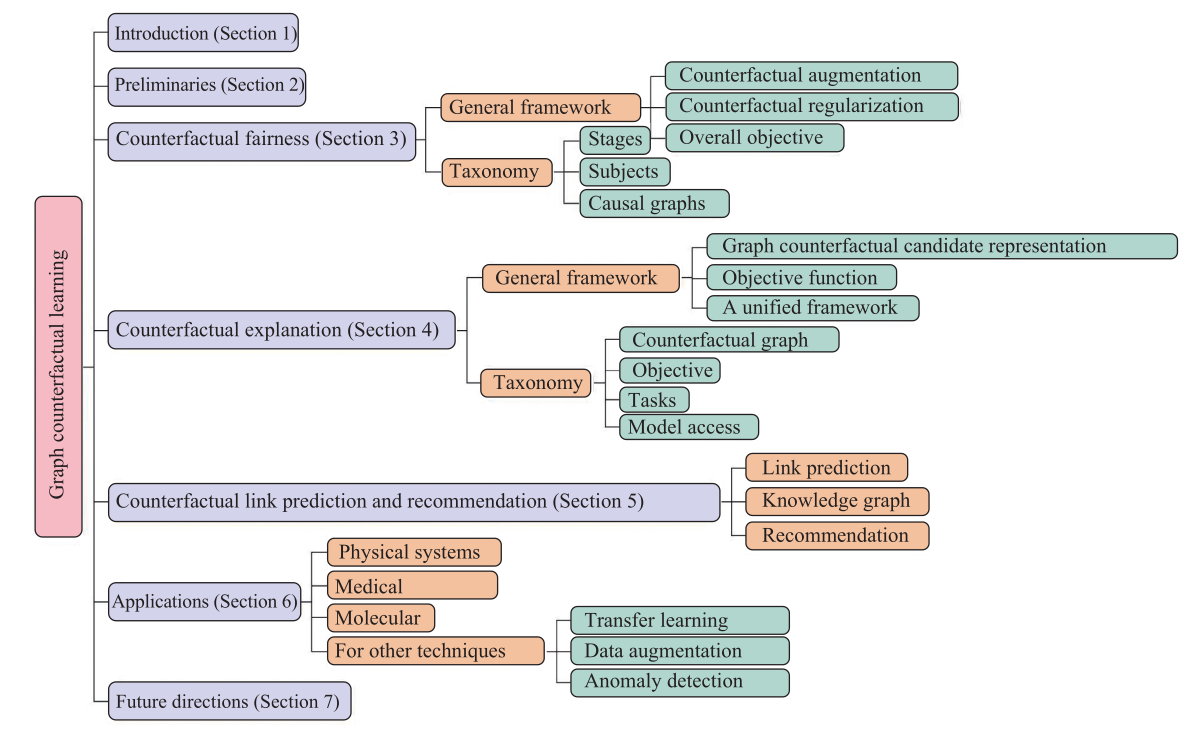
\includegraphics[width=0.8\linewidth]{paper_structure.png}
		\end{figure}
	\end{frame}
	%------------------------------------------------
	\section{Counterfactual Fairness}
	%------------------------------------------------
	
	\begin{frame}{Sources of Bias}
		\begin{itemize}
		\item	The biases in the data lead to unfair predictions
		\item Various sources of bias in any i.i.d (independent and identically distributed data)
			\begin{enumerate}
				\item Historical Bias
				\item Representation Bias
				\item Temporal Bias
				\item Attribute Bias				
			\end{enumerate}
			\item Source of Bias specific to graph data
			\begin{enumerate}
				\item Linking Bias
				\item Structural Bias
			\end{enumerate}
		\end{itemize}
		
	\end{frame}
	
	%------------------------------------------------
	
	\begin{frame}{Counterfactual Fairness}
		
		\begin{itemize}
			\item Biases are measured from different perspectives. 
			\begin{enumerate}
				\item Group fairness 
				\item Individual fairness
			\end{enumerate}
			\item The above metrics rely on the statistical correlation among variables, which may not describe the intrinsic causal structure
			\item Inspired by the development of counterfactual learning, counterfactual fairness is proposed as a notion to measure fairness from the perspective of causal inference
		\end{itemize}
		\begin{block}{Definition}
			Counterfactual fairness makes the outputs of a machine learning model for an individual in the actual world remain the same when we flip the sensitive attribute of the same individual to the counterfactual world.
		\end{block}
		
		

	\end{frame}
	
	%------------------------------------------------
	
	\begin{frame}{Multiple Columns}
		\begin{columns}[c] % The "c" option specifies centered vertical alignment while the "t" option is used for top vertical alignment
			
			\column{.45\textwidth} % Left column and width
			\textbf{Heading}
			\begin{enumerate}
				\item Statement
				\item Explanation
				\item Example
			\end{enumerate}
			
			\column{.45\textwidth} % Right column and width
			Lorem ipsum dolor sit amet, consectetur adipiscing elit. Integer lectus nisl, ultricies in feugiat rutrum, porttitor sit amet augue. Aliquam ut tortor mauris. Sed volutpat ante purus, quis accumsan dolor.
			
		\end{columns}
	\end{frame}
	
	%------------------------------------------------
	\section{Counterfactual Learning}
	%------------------------------------------------
	\begin{frame}{Counterfactual Learning}
		\begin{itemize}
			\item Counterfactual learning gives a chance to alleviate the intrinsic bias making models interpretable and exploiting the information stored in data well
			\item Counterfactual comes from the research community of causal inference. 
			\item 2 main concepts
			\begin{enumerate}
				\item Counterfactual Fairness: prediction for an individual is 			fair if it remains the same in a counterfactual world where the individual belongs to a different demographic	group
				\item Counterfactual Explanation
			\end{enumerate}
			\item Besides the aid on fairness and interpretability, the research community also utilizes counterfactual learning to provide additional information from the counterfactual world \cite{p1}
		\end{itemize}
	\end{frame}
	\begin{frame}{Counterfactual Learning cont..}
		\begin{itemize}
			\item Compared with traditional statistical models, causal 		models have better generalization ability in modeling real-world systems
		\end{itemize}
	\end{frame}
	\begin{frame}{Counterfactual Learning}
		\begin{table}
			\begin{tabular}{l l l}
				\toprule
				\textbf{Treatments} & \textbf{Response 1} & \textbf{Response 2} \\
				\midrule
				Treatment 1         & 0.0003262           & 0.562               \\
				Treatment 2         & 0.0015681           & 0.910               \\
				Treatment 3         & 0.0009271           & 0.296               \\
				\bottomrule
			\end{tabular}
			\caption{Table caption}
		\end{table}
	\end{frame}
	
	%------------------------------------------------
	
	\begin{frame}{Theorem}
		\begin{theorem}[Mass--energy equivalence]
			$E = mc^2$
		\end{theorem}
	\end{frame}
	
	%------------------------------------------------
	
	\begin{frame}{Figure}
		Uncomment the code on this slide to include your own image from the same directory as the template .TeX file.
		%\begin{figure}
		%\includegraphics[width=0.8\linewidth]{test}
		%\end{figure}
	\end{frame}
	
	
	
	\section{Counterfactual Learning on Graphs}
	\begin{frame}{Counterfactual Learning on Graphs}
		\begin{itemize}
			\item Recent works on graph counterfactual learning have shown great potential to overcome the aforementioned challenges 	on fairness, explanation, etc.
		\end{itemize}
	\end{frame}
	%------------------------------------------------
	
	\begin{frame}[fragile] % Need to use the fragile option when verbatim is used in the slide
		\frametitle{Citation}
		An example of the \verb|\cite| command to cite within the presentation:\\~
		
		This statement requires citation \cite{p1}.
	\end{frame}
	
	%------------------------------------------------
	
	\begin{frame}{References}
		\footnotesize
		\bibliography{reference.bib}
		\bibliographystyle{apalike}
	\end{frame}
	
	%------------------------------------------------
	
	
	\begin{frame}
		\Huge{\centerline{\textbf{The End}}}
	\end{frame}
	
	%----------------------------------------------------------------------------------------
	
\end{document}
